\documentclass[11pt]{article}
\usepackage[margin=0.82in]{geometry}
\usepackage[T1]{fontenc}
\usepackage{lmodern}
\usepackage{amsmath,amssymb,booktabs,graphicx,float,longtable,microtype,tabularx,xcolor,listings,fancyhdr,tikz,tcolorbox,titlesec,enumitem}
\tcbuselibrary{breakable}
\usetikzlibrary{arrows.meta,positioning,matrix}
\usepackage{xurl}
\usepackage[colorlinks=true,urlcolor=blue!55!black,linkcolor=blue!55!black]{hyperref}
\graphicspath{{../../output/llm/figures/}}
\definecolor{navy}{HTML}{1F4E78}
\definecolor{coral}{HTML}{E07A5F}
\definecolor{teal}{HTML}{2A9D8F}
\definecolor{codebg}{HTML}{F3F6F8}
\titleformat{\section}{\Large\bfseries\color{navy}}{\thesection}{0.7em}{}
\titleformat{\subsection}{\large\bfseries\color{teal!65!black}}{\thesubsection}{0.7em}{}
\newtcolorbox{studybox}[1]{breakable,colback=navy!4,colframe=navy!55,
  title={#1},fonttitle=\bfseries,boxrule=0.5pt,arc=1.5mm,
  left=7pt,right=7pt,top=5pt,bottom=5pt}
\setlist{itemsep=2pt,topsep=4pt}
\setcounter{tocdepth}{2}
\setlength{\emergencystretch}{2em}
\newcolumntype{P}[1]{>{\raggedright\arraybackslash}p{#1}}
\raggedbottom
\setlength{\parindent}{0pt}
\setlength{\parskip}{5pt}
\pagestyle{fancy}
\setlength{\headheight}{14pt}
\fancyhf{}
\lhead{MATH 550 -- LLMs from Scratch}
\rhead{\thepage}
\lstset{basicstyle=\ttfamily\small,backgroundcolor=\color{codebg},frame=single,
  rulecolor=\color{navy!25},breaklines=true,columns=fullflexible,
  showstringspaces=false,keepspaces=true,tabsize=4,
  keywordstyle=\color{navy}\bfseries,commentstyle=\color{teal!60!black},
  stringstyle=\color{coral!70!black},aboveskip=9pt,belowskip=8pt}
% Every example is short enough for one page. Keep complete code together.
\BeforeBeginEnvironment{lstlisting}{\par\noindent\begin{minipage}{\linewidth}}
\AfterEndEnvironment{lstlisting}{\end{minipage}\par}
\newcommand{\E}{\mathbb{E}}
\newcommand{\softmax}{\operatorname{softmax}}
\newcommand{\bookrepo}{https://github.com/rasbt/LLMs-from-scratch/blob/f49cad747931fe6af0a7d2802cd480d1c1a0ec8e}
\newcommand{\booklink}[2]{\href{\bookrepo/#1}{#2}}
\hypersetup{pdftitle={Build Large Language Models from Scratch},
  pdfauthor={MATH 550},pdfsubject={GPT-2 pretraining and post-training extensions}}
\title{\color{navy}\textbf{Large Language Models from Scratch}\\
\large A guided implementation of GPT-2 pretraining\\[3pt]}
\author{MATH 550 Mathematical Data Science Capstone}
\date{}

\begin{document}
\maketitle
\begin{studybox}{How to use these notes}
Read Part I alongside Sebastian Raschka's \emph{Build a Large Language Model
(From Scratch)} (Manning, 2024). The teaching order follows chapters 2--5:
text and batches, attention, the GPT decoder, and pretraining. The explanations,
worked examples, and diagrams here are original course material rather than a
reproduction of the book. Part II retains instruction-tuning and RLHF lessons.
\end{studybox}
\tableofcontents
\clearpage

\section{Learning route and scope}

The goal is to make the complete causal-language-model pipeline inspectable.
Students build the tokenizer, decoder, objectives, data packing, optimization,
generation, supervised fine-tuning (SFT), pairwise reward model, and a compact
reinforcement-learning-from-human-feedback (RLHF) loop. PyTorch supplies tensor
operations, standard layers, automatic differentiation, and optimizers. The
local course module does not import a pretrained model, a pretrained tokenizer,
\texttt{torch.nn.Transformer}, or a GPT/Transformer training framework.
Raschka's main chapter code instead uses the existing GPT-2 BPE tokenizer via
\texttt{tiktoken}; this is a deliberate difference, not a model-architecture
shortcut. Both routes make the decoder and its training computation explicit.

The resulting checkpoints are teaching models. Our archived public-book example
used a corpus with about eight million training tokens, but its 30-update run
consumed only a small sampled portion. It demonstrated the training pipeline,
not complete training on that corpus. It cannot reproduce the factual breadth, safety work,
multilingual coverage, or compute of a production assistant. A falling loss is
evidence that an objective is being optimized; it is not evidence of truth,
reasoning, harmlessness, or usefulness.

\subsection*{Learning objectives}
By the end of nine lecture/studio units, students should be able to:
\begin{enumerate}
\item explain UTF-8 byte tokenization and derive the BPE merge procedure;
\item derive causal next-token maximum likelihood and connect it to cross-entropy;
\item track every tensor shape through multi-head causal self-attention;
\item implement and test a GPT-style decoder in elementary PyTorch;
\item design a leakage-resistant pretraining split and interpret held-out loss;
\item construct assistant-only SFT labels and diagnose prompt-loss leakage;
\item derive the Bradley--Terry pairwise reward objective;
\item derive KL-shaped rewards, generalized advantage estimation (GAE), and
the clipped proximal policy optimization (PPO) objective; and
\item audit data rights, memorization, reward hacking, historical bias, and the
gap between a classroom experiment and a production LLM.
\end{enumerate}

\subsection{Book-to-course map}
The chapter notebooks are the primary reference; the shorter companion scripts
occasionally use different hyperparameters. Links below are pinned to repository
revision
\begin{center}\texttt{f49cad747931fe6af0a7d2802cd480d1c1a0ec8e}.\end{center}
This is the same revision used for the GPT-2 slide deck, keeping reading
assignments stable.
\begin{center}\small
\begin{tabularx}{\linewidth}{@{}p{0.17\linewidth}XX@{}}
\toprule
Reading & Main construction & Local course adaptation \\
\midrule
\booklink{ch02/01_main-chapter-code/ch02.ipynb}{Chapter 2} & Token IDs, GPT-2 BPE, shifted windows, token/position embeddings & Train a smaller byte-level BPE on training books. \\
\booklink{ch03/01_main-chapter-code/ch03.ipynb}{Chapter 3} & Simple attention, learned Q/K/V, causal masking, multiple heads & Fuse the three projections in one linear layer. \\
\booklink{ch04/01_main-chapter-code/ch04.ipynb}{Chapter 4} & LayerNorm, GELU, residual blocks, complete GPT & Use tied embeddings and smaller device presets. \\
\booklink{ch05/01_main-chapter-code/ch05.ipynb}{Chapter 5} & Loss/evaluation, first training loop, sampling, checkpoints & Scale to whole-book holdouts and memory-mapped token streams. \\
\booklink{appendix-D/01_main-chapter-code/appendix-D.ipynb}{Appendix D} & Warmup, cosine decay, gradient clipping & Add accumulation, tokenizer checks, and optional DDP. \\
\bottomrule
\end{tabularx}\end{center}

\subsection{Nine-unit course map}
\begin{longtable}{@{}P{0.05\linewidth}P{0.21\linewidth}P{0.42\linewidth}P{0.21\linewidth}@{}}
\toprule
Unit & Central question & Main ideas and studio & Evidence of learning \\
\midrule
\endhead
1 & What is a token? & Unicode, UTF-8 bytes, special tokens, BPE frequency table,
round-trip and compression tests. & Train and serialize a tokenizer. \\
2 & Why next-token prediction? & Chain rule, teacher forcing, cross-entropy,
bigram baseline, train/validation leakage. & Derive and fit the baseline. \\
3 & How can a token use context? & Embeddings, queries, keys, values, scale,
causal mask, multiple heads. & Shape trace and future-token invariance test. \\
4 & What makes GPT a trainable system? & Pre-norm blocks, residual paths, MLP,
position embeddings, initialization, tied weights. & Implement a forward/backward pass. \\
5 & What does pretraining evidence mean? & First a minimal AdamW loop, loss,
perplexity, sampling, and checkpoints; then schedules and hardware extensions. & Run public books and compare bigram. \\
6 & Why does a base model not follow instructions? & Prompt template, SFT,
assistant-only mask, padding, truncation, held-out prompts. & Fine-tune on Dolly 15k. \\
7 & How can preferences become a scalar? & Chosen/rejected pairs, reward head,
Bradley--Terry likelihood, pair accuracy, distribution shift. & Train and audit a reward model. \\
8 & Where is the reinforcement learning? & Rollouts, reference policy, token KL,
state values, GAE, PPO clipping, entropy. & Execute and test one PPO update. \\
9 & What would justify a claim? & Memorization, reward hacking, unsafe data,
human evaluation, data rights, scaling limits. & Model card and evidence audit. \\
\bottomrule
\end{longtable}

\clearpage
\part{The book-aligned pretraining path}
\section{Text, training windows, and embeddings: chapter 2}
\label{sec:text}

\subsection{Token IDs are not token vectors}
The preprocessing pipeline turns text into a sequence of integer IDs. A learned
embedding layer then maps those IDs to vectors. Tokenization determines the
prediction alphabet; embedding coordinates are model parameters learned during
pretraining. A token may be a complete word, a word fragment, punctuation, or a
byte-related unit. Whitespace affects tokenization, so the tokens for a word in
isolation need not match those for the same letters after a space.

Raschka first builds simple tokenizers to expose splitting, vocabulary lookup,
unknown tokens, and special tokens, then uses GPT-2 byte-pair encoding (BPE).
The main code uses a vocabulary of $50{,}257$, obtained with
\texttt{tiktoken.get\_encoding("gpt2")}. Using that tokenizer does not load
any pretrained GPT weights.
The local course route below trains a smaller tokenizer and is not compatible
with the released GPT-2 vocabulary.

\subsection{Course extension: learning byte-pair merges}

Computers receive text as bytes. UTF-8 maps every Unicode string to a sequence
in $\{0,\ldots,255\}^*$. A byte tokenizer is therefore lossless and has no
unknown token. Its weakness is sequence length: a frequent English word may use
several tokens, and a non-ASCII character often uses several bytes.

Byte-pair encoding starts with the 256 byte symbols. Within simple regex
pre-tokens, count every adjacent pair, merge the most frequent pair, assign a new
integer ID, and repeat. If $c(s)$ is the frequency of token sequence $s$, then
the score of pair $(a,b)$ is
\[
C(a,b)=\sum_s c(s)\sum_{i=1}^{|s|-1}
\mathbf{1}\{(s_i,s_{i+1})=(a,b)\}.
\]
Training stores an ordered list of merges. Encoding must apply the available
merge with smallest training rank, not merely the pair that happens to appear
most often in a new string. Decoding concatenates the byte strings represented
by the final token IDs and then performs UTF-8 decoding.

The course reserves five non-byte control tokens: end-of-text, pad, system,
user, and assistant. The archived small experiment used 512 entries: 256 raw
bytes, five control tokens, and 251 learned merges. This is an experiment
setting, not a fixed requirement; a later 10,000-entry request may produce a
larger actual vocabulary. Fit the tokenizer on training books only.
Fitting it on validation books would leak their spelling and frequency
structure into the model-selection process.

The requested BPE size is an upper bound. Training stops before that bound if no
remaining pair meets the minimum frequency, so the saved tokenizer and corpus
metadata record the actual vocabulary size. The standard pretraining drivers use
that actual size directly. A customized model may instead round its embedding
and output tables upward for hardware alignment; those extra rows are model
parameters, not decodable tokens.

\subsection*{Tokenizer checks}
\begin{itemize}
\item Unicode round trip: \texttt{decode(encode(text)) == text}.
\item Determinism: identical text and settings produce identical merge ranks.
\item Serialization: a saved and reloaded tokenizer produces identical IDs.
\item Compression: repeated common substrings use fewer BPE tokens than bytes.
\item Boundary rule: merges never cross the declared pre-token boundary.
\end{itemize}

\subsection{One-token shifts create the training targets}
Given token stream $[11,7,23,5,9,4]$ and context length $T=4$, the first input
window is $[11,7,23,5]$ and its target is $[7,23,5,9]$. Thus the model predicts a
next token at \emph{every} input position, not only at the end of the window.
Raschka's \texttt{GPTDatasetV1} packages these pairs and a PyTorch DataLoader
batches them. With stride $s$, successive starting indices differ by $s$.
Stride $1$ gives heavily overlapping windows; stride $T$ gives nonoverlapping
input windows. In either case targets remain shifted by exactly one token.

\begin{lstlisting}[language=Python]
ids = torch.tensor([11, 7, 23, 5, 9, 4], dtype=torch.long)
T, stride = 4, 1
pairs = [(ids[i:i+T], ids[i+1:i+T+1])
         for i in range(0, len(ids) - T, stride)]
X = torch.stack([x for x, y in pairs])  # (2, 4)
Y = torch.stack([y for x, y in pairs])  # (2, 4)
\end{lstlisting}

A context of $T$ tokens needs $T+1$ consecutive tokens to form all its labels.
Windows without all $T$ targets are dropped in this example. The causal mask
and the shift solve different problems: the shift specifies the prediction
target, while the mask prevents the network from reading that target as a
future input. Unshifted targets permit trivial copying of the visible token.

\subsection{Token lookup plus position lookup}
For vocabulary size $V$, model width $d$, and maximum context $C$, learn tables
$E_{\rm tok}\in\mathbb R^{V\times d}$ and
$E_{\rm pos}\in\mathbb R^{C\times d}$. For a batch of IDs of shape $(B,T)$,
\[
H^{(0)}_{b,t}=E_{\rm tok}[x_{b,t}]+E_{\rm pos}[t],
\qquad H^{(0)}\in\mathbb R^{B\times T\times d},\quad T\le C.
\]
Positions are indexed $0,\ldots,T-1$ in code. Mathematical examples below use
positions $1,\ldots,T$ when convenient. The position table is learned, rather
than sinusoidal or rotary, in this GPT-2 architecture.
\begin{lstlisting}[language=Python]
tok_emb = nn.Embedding(V, d)
pos_emb = nn.Embedding(C, d)
positions = torch.arange(X.shape[1], device=X.device)
h = tok_emb(X) + pos_emb(positions)  # broadcast over B
\end{lstlisting}

\begin{studybox}{Check your understanding}
For stream $[3,1,4,1,5]$ and $T=3$, write the first input and target. Then give
the embedding output shape when $B=2$ and $d=8$. Explain why an ID must be an
integer, but an embedding coordinate can change continuously during training.
\end{studybox}

\section{Causal multi-head self-attention: chapter 3}
\label{sec:attention}

Attention is a differentiable retrieval operation. A query describes what the
current position is looking for; keys describe what each memory position can be
matched on; values contain the information that will be combined. Figure
\ref{fig:attention-retrieval} separates these roles before introducing the
special case used by GPT.
Raschka first computes attention directly from small input vectors, then adds
learned query, key, and value maps. Follow that order when implementing: verify
one query and its weights before introducing a batch, a mask, or multiple heads.

\begin{figure}[H]
\centering
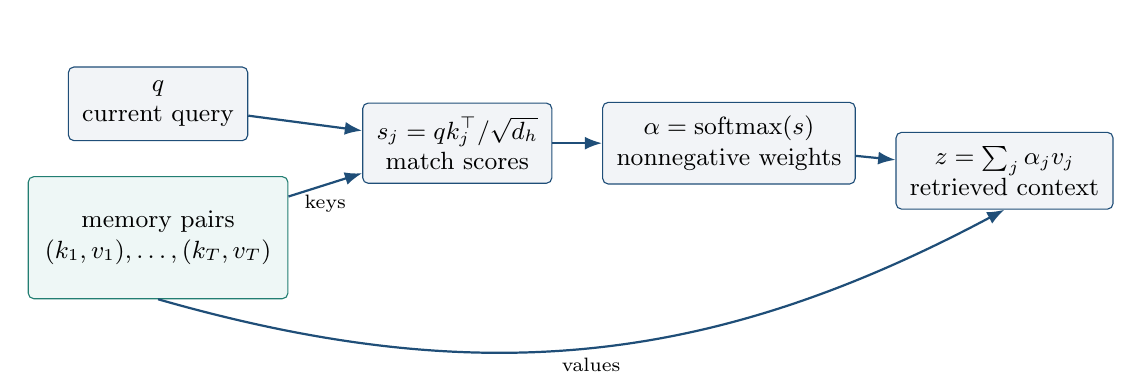
\begin{tikzpicture}[
  >=Latex,
  flow/.style={-{Latex[length=2.2mm]},thick,draw=navy},
  box/.style={draw=navy,rounded corners=2pt,fill=navy!6,
    minimum height=0.9cm,align=center,font=\small,inner sep=5pt},
  memory/.style={draw=teal!80!black,rounded corners=2pt,fill=teal!8,
    minimum height=1.55cm,align=center,font=\small,inner sep=6pt}
]
\node[box] (query) at (0,0.85) {$q$\\current query};
\node[memory] (memory) at (0,-0.85) {memory pairs\\
  $(k_1,v_1),\ldots,(k_T,v_T)$};
\node[box] (scores) at (3.8,0.35) {$s_j=qk_j^\top/\sqrt{d_h}$\\match scores};
\node[box] (weights) at (7.25,0.35) {$\alpha=\softmax(s)$\\nonnegative weights};
\node[box] (output) at (10.75,0) {$z=\sum_j\alpha_jv_j$\\retrieved context};
\draw[flow] (query) -- (scores);
\draw[flow] (memory) -- node[below,font=\scriptsize]{keys} (scores);
\draw[flow] (scores) -- (weights);
\draw[flow] (weights) -- (output);
\draw[flow] (memory.south) to[bend right=22]
  node[below,font=\scriptsize]{values} (output.south);
\end{tikzpicture}
\caption{Attention as soft retrieval. Similarity between the query and each key
sets the mixture weight on the corresponding value. Queries and memory may come
from different sources, so attention is not automatically self-attention.}
\label{fig:attention-retrieval}
\end{figure}

Let $X\in\mathbb R^{B\times T\times d}$ be a batch of hidden states. We treat
feature vectors as rows, so matrices multiply on the right. Separate learned
maps produce $Q,K,V$; the course stores them in one equivalent fused linear
layer. Reshape the projected width into $H$ heads of width $d_h=d/H$:
\[
Q=XW_Q,\qquad K=XW_K,\qquad V=XW_V.
\]
Bias terms are omitted in this equation. The course enables them by default;
the book's initial attention configuration disables them.
For one head,
\[
S=\frac{QK^\top}{\sqrt{d_h}}+M,\qquad
P=\softmax(S),\qquad A=PV,
\]
where $M_{ij}=0$ for $j\le i$ and $M_{ij}=-\infty$ for $j>i$. The scale
$\sqrt{d_h}$ stabilizes score variance under a simple independence model:
if coordinates of $q$ and $k$ are independent, mean zero, and variance one,
then $\operatorname{Var}(qk^\top)=d_h$. Dividing by $\sqrt{d_h}$ gives variance
one under those assumptions. Learned vectors need not satisfy them exactly.
Softmax acts across \emph{keys}, the last score dimension. The mask makes the
model causal. Apply attention-weight dropout during training, mix the values,
concatenate all heads, and apply the output projection and branch dropout.

In \emph{self-attention}, every query, key, and value is projected from the same
input sequence $X$. The operation still uses three learned projections because
matching and content transport are different jobs. Figure
\ref{fig:self-attention-flow} shows the full tensor path for one head; multiple
heads repeat this path with different learned subspaces and concatenate their
outputs.

\begin{figure}[H]
\centering
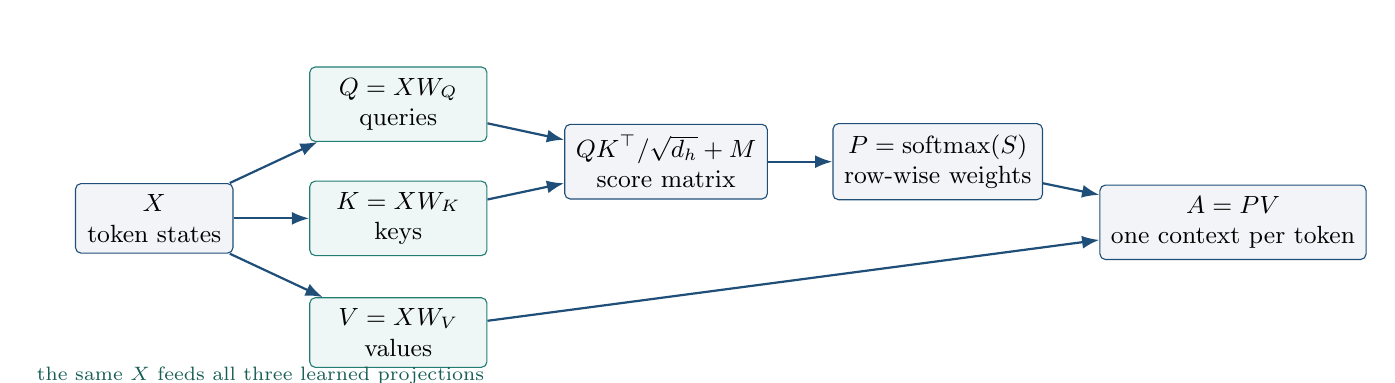
\begin{tikzpicture}[
  >=Latex,
  flow/.style={-{Latex[length=2.2mm]},thick,draw=navy},
  box/.style={draw=navy,rounded corners=2pt,fill=navy!6,
    minimum height=0.82cm,minimum width=2.0cm,align=center,font=\small,inner sep=4pt},
  projection/.style={draw=teal!80!black,rounded corners=2pt,fill=teal!8,
    minimum height=0.82cm,minimum width=2.25cm,align=center,font=\small,inner sep=4pt}
]
\node[box] (x) at (0,0) {$X$\\token states};
\node[projection] (q) at (3.1,1.45) {$Q=XW_Q$\\queries};
\node[projection] (k) at (3.1,0) {$K=XW_K$\\keys};
\node[projection] (v) at (3.1,-1.45) {$V=XW_V$\\values};
\node[box] (score) at (6.5,0.72) {$QK^\top/\sqrt{d_h}+M$\\score matrix};
\node[box] (prob) at (9.95,0.72) {$P=\softmax(S)$\\row-wise weights};
\node[box] (context) at (13.7,-0.05) {$A=PV$\\one context per token};
\draw[flow] (x) -- (q);
\draw[flow] (x) -- (k);
\draw[flow] (x) -- (v);
\draw[flow] (q) -- (score);
\draw[flow] (k) -- (score);
\draw[flow] (score) -- (prob);
\draw[flow] (prob) -- (context);
\draw[flow] (v) -- (context);
\node[font=\scriptsize,text=teal!60!black,align=center] at (1.35,-2.0)
  {the same $X$ feeds all three learned projections};
\end{tikzpicture}
\caption{Self-attention for one head. The $T\times T$ matrix contains one row
of attention weights for each query position and one column for each key/value
position. The weighted values produce a new contextual representation at every
token position.}
\label{fig:self-attention-flow}
\end{figure}

GPT uses \emph{masked self-attention}, more precisely causal self-attention. The
mask is added to the score matrix before softmax. For query position $i$, keys
at $j>i$ receive $-\infty$, so their probability is exactly zero. This permits
parallel teacher-forced training without allowing a position to read its target
or any later token.

\begin{figure}[H]
\centering
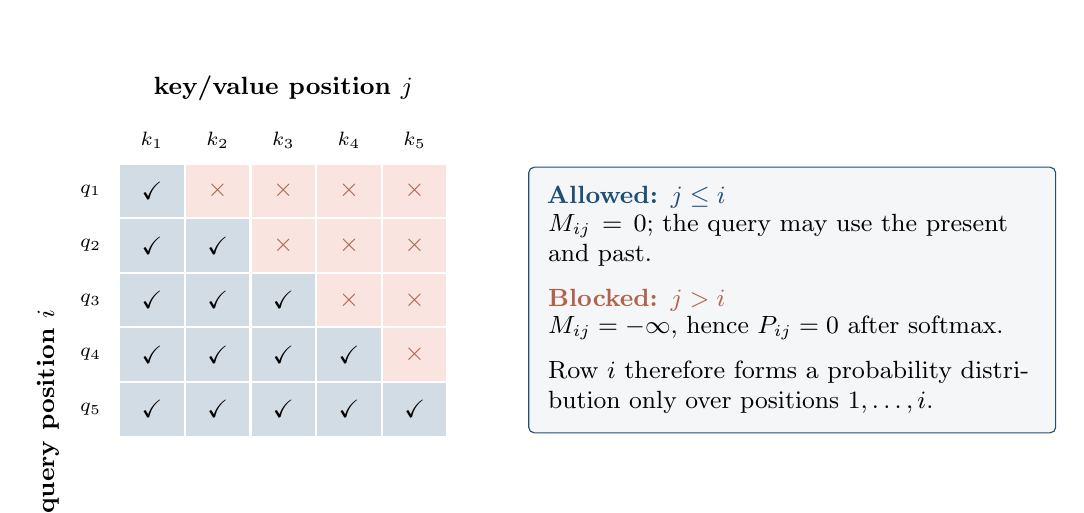
\begin{tikzpicture}[
  cell/.style={minimum width=0.82cm,minimum height=0.68cm,
    anchor=center,draw=white,font=\small},
  explainer/.style={draw=navy,rounded corners=2pt,fill=navy!5,
    text width=6.2cm,align=left,font=\small,inner sep=7pt}
]
\matrix (mask) [matrix of math nodes,row sep=0pt,column sep=0pt] {
|[cell,fill=navy!20]| \checkmark & |[cell,fill=coral!20,text=coral!80!black]| \times & |[cell,fill=coral!20,text=coral!80!black]| \times & |[cell,fill=coral!20,text=coral!80!black]| \times & |[cell,fill=coral!20,text=coral!80!black]| \times \\
|[cell,fill=navy!20]| \checkmark & |[cell,fill=navy!20]| \checkmark & |[cell,fill=coral!20,text=coral!80!black]| \times & |[cell,fill=coral!20,text=coral!80!black]| \times & |[cell,fill=coral!20,text=coral!80!black]| \times \\
|[cell,fill=navy!20]| \checkmark & |[cell,fill=navy!20]| \checkmark & |[cell,fill=navy!20]| \checkmark & |[cell,fill=coral!20,text=coral!80!black]| \times & |[cell,fill=coral!20,text=coral!80!black]| \times \\
|[cell,fill=navy!20]| \checkmark & |[cell,fill=navy!20]| \checkmark & |[cell,fill=navy!20]| \checkmark & |[cell,fill=navy!20]| \checkmark & |[cell,fill=coral!20,text=coral!80!black]| \times \\
|[cell,fill=navy!20]| \checkmark & |[cell,fill=navy!20]| \checkmark & |[cell,fill=navy!20]| \checkmark & |[cell,fill=navy!20]| \checkmark & |[cell,fill=navy!20]| \checkmark \\
};
\foreach \j in {1,...,5}
  \node[above=2pt of mask-1-\j,font=\scriptsize] {$k_{\j}$};
\foreach \i in {1,...,5}
  \node[left=3pt of mask-\i-1,font=\scriptsize] {$q_{\i}$};
\node[above=0.55cm of mask,font=\small\bfseries] {key/value position $j$};
\node[rotate=90,left=0.78cm of mask,font=\small\bfseries] {query position $i$};
\node[explainer,right=0.9cm of mask] (legend) {
  \textcolor{navy}{\textbf{Allowed: $j\le i$}}\\[-1pt]
  $M_{ij}=0$; the query may use the present and past.\\[5pt]
  \textcolor{coral!80!black}{\textbf{Blocked: $j>i$}}\\[-1pt]
  $M_{ij}=-\infty$, hence $P_{ij}=0$ after softmax.\\[5pt]
  Row $i$ therefore forms a probability distribution only over positions
  $1,\ldots,i$.
};
\end{tikzpicture}
\caption{The lower-triangular causal mask. Blue cells are visible; coral cells
are future positions excluded before softmax. The diagonal remains visible so a
hidden state at position $i$ can represent token $x_i$ while predicting
$x_{i+1}$.}
\label{fig:causal-mask}
\end{figure}

\subsection{A masked row worked by hand}
Suppose the already-scaled scores for query position $2$ are $[1,2,9]$. The
third key is in the future, so replace its score by $-\infty$ before softmax:
\[
P_{2,:}=\frac{[e^1,e^2,0]}{e^1+e^2}
\approx[0.268941,0.731059,0].
\]
For values $v_1=[2,0]$ and $v_2=[0,4]$, the contextual vector is
\[
a_2=0.268941[2,0]+0.731059[0,4]
\approx[0.537883,2.924234].
\]
Softmax followed by zeroing the third probability would leave a row whose
entries no longer sum to one. Masking first changes the normalization set.
The row-sum-one invariant applies before dropout or in evaluation mode;
attention dropout does not preserve each realized row sum during training.

\subsection{Split and merge heads explicitly}

\begin{center}
\begin{tabular}{lll}
\toprule
Tensor & Shape & Meaning \\
\midrule
$X$ & $B\times T\times d$ & contextual token states \\
$Q,K,V$ & $B\times H\times T\times d_h$ & per-head projections \\
$S,P$ & $B\times H\times T\times T$ & causal scores and weights \\
$A$ & $B\times H\times T\times d_h$ & per-head weighted values \\
output & $B\times T\times d$ & concatenated, projected result \\
\bottomrule
\end{tabular}
\end{center}

The following core uses $H\mid d$. It assumes \texttt{self.qkv} is
\texttt{nn.Linear(d, 3*d)}. The full attention module also includes dropout
and the output projection; they are omitted here to isolate the tensor path.
\begin{lstlisting}[language=Python]
B, T, d = x.shape
q, k, v = self.qkv(x).chunk(3, dim=-1)
def split(z):
    return z.view(B, T, H, d // H).transpose(1, 2)
q, k, v = map(split, (q, k, v))
scores = (q @ k.transpose(-2, -1)) / math.sqrt(d // H)
keep = torch.ones(T, T, device=x.device).tril().bool()
weights = scores.masked_fill(~keep, -torch.inf).softmax(-1)
context = (weights @ v).transpose(1, 2).contiguous()
context = context.view(B, T, d)
\end{lstlisting}

The most important unit test changes tokens at positions $j\ge k$ and verifies
that logits at positions $i<k$ do not change. This is stronger than merely
checking that the mask has a triangular shape: it tests the behavior of the
complete model. Put the model in evaluation mode first, so independent dropout
masks do not obscure the comparison. In the local implementation compare
\texttt{model(ids).logits}, since forward returns a \texttt{GPTOutput} object.

For one sequence, attention mixing costs $O(T^2d)$ time. Explicit score storage
has $BHT^2$ entries; projection and MLP computation add terms proportional to
$BTd^2$. The accelerator presets use $T=256$ (smoke: 64; CPU: 128).
Production systems use
fused kernels, longer-context methods, and caching; those
optimizations remain outside the core model implementation. An optional DDP
training driver is included as a readable systems extension.

\section{The complete GPT decoder: chapter 4}
\label{sec:decoder}

Attention supplies context mixing, but a trainable decoder also needs
normalization, nonlinear feature transformations, and residual paths. Raschka
builds these components individually before assembling \texttt{GPTModel}.

\subsection{Layer normalization and the feed-forward network}
For one token vector $h\in\mathbb R^d$, layer normalization computes statistics
across its $d$ features, not across examples or sequence positions:
\[
\mu=\frac1d\sum_{j=1}^d h_j,\quad
\sigma^2=\frac1d\sum_{j=1}^d(h_j-\mu)^2,\quad
\operatorname{LN}(h)=\gamma\odot\frac{h-\mu}{\sqrt{\sigma^2+\epsilon}}+\beta.
\]
Use population variance and $\epsilon=10^{-5}$. Learned vectors $\gamma,\beta$
have width $d$. The book spells out the calculation; the local module uses
\texttt{nn.LayerNorm}. Both expose the same feature-wise operation.

The token-wise multilayer perceptron (MLP) expands width from $d$ to $4d$, applies
GELU, and returns to width $d$:
\[
\operatorname{MLP}(h)=\operatorname{GELU}(hW_1+b_1)W_2+b_2.
\]
Here $W_1\in\mathbb R^{d\times4d}$ and $W_2\in\mathbb R^{4d\times d}$;
\texttt{nn.Linear.weight} stores their transposes. GPT-2 uses the approximation
\[
\operatorname{GELU}(u)\approx\tfrac12u\left[1+\tanh\left(
\sqrt{2/\pi}(u+0.044715u^3)\right)\right],
\]
applied coordinate-wise. Attention mixes positions; the same MLP transforms
features independently at each position. \texttt{nn.GELU(approximate="tanh")}
implements this choice in the course module.

\subsection{Pre-normalized residual blocks}

Token and learned position embeddings are added:
\[
H^{(0)}_{b,t}=E_{\mathrm{tok}}[x_{b,t}]+E_{\mathrm{pos}}[t].
\]
Each pre-normalized block is
\begin{align*}
U^{(\ell)} &= H^{(\ell-1)}+\operatorname{Attn}
(\operatorname{LN}(H^{(\ell-1)})),\\
H^{(\ell)} &= U^{(\ell)}+\operatorname{MLP}
(\operatorname{LN}(U^{(\ell)})),
\end{align*}
where branch dropout is suppressed in the equations. Each branch must return
shape $(B,T,d)$ so the addition is defined. The derivative of a residual map
$h+f(h)$ contains $I+J_f(h)$; the identity path helps gradients travel through
the stack but does not by itself guarantee stable optimization.
% Original course diagram. Each skip starts at the input of its own branch.
\begin{figure}[H]
\centering
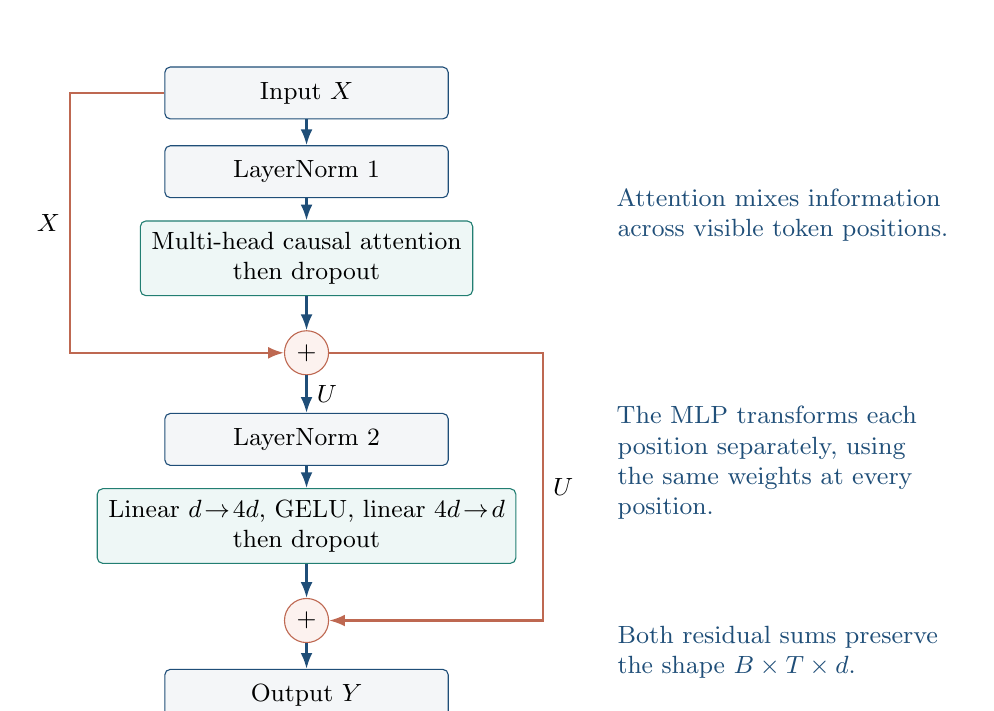
\begin{tikzpicture}[
  font=\small,
  flow/.style={-{Latex[length=2mm]},thick,draw=navy},
  skip/.style={-{Latex[length=2mm]},thick,draw=coral!85!black},
  box/.style={draw=navy,fill=navy!5,rounded corners=2pt,
    minimum width=3.6cm,minimum height=0.66cm,align=center,inner sep=4pt},
  operation/.style={box,draw=teal!80!black,fill=teal!8,minimum height=0.9cm},
  add/.style={circle,draw=coral!85!black,fill=coral!10,
    minimum size=0.56cm,inner sep=0pt},
  explanation/.style={align=left,text width=4.3cm,text=navy}
]
\node[box] (input) at (0,0) {Input $X$};
\node[box] (norm1) at (0,-1.0) {LayerNorm 1};
\node[operation] (attn) at (0,-2.1)
  {Multi-head causal attention\\then dropout};
\node[add] (add1) at (0,-3.3) {$+$};
\node[box] (norm2) at (0,-4.4) {LayerNorm 2};
\node[operation,minimum width=4.3cm] (mlp) at (0,-5.5)
  {Linear $d\!\to\!4d$, GELU, linear $4d\!\to\!d$\\then dropout};
\node[add] (add2) at (0,-6.7) {$+$};
\node[box] (output) at (0,-7.65) {Output $Y$};

\draw[flow] (input) -- (norm1);
\draw[flow] (norm1) -- (attn);
\draw[flow] (attn) -- (add1);
\draw[flow] (add1) -- node[right] {$U$} (norm2);
\draw[flow] (norm2) -- (mlp);
\draw[flow] (mlp) -- (add2);
\draw[flow] (add2) -- (output);

% The first bypass carries X; the second carries the updated state U.
\draw[skip] (input.west) -- (-3,0)
  -- node[left] {$X$} (-3,-3.3) -- (add1.west);
\draw[skip] (add1.east) -- (3,-3.3)
  -- node[right] {$U$} (3,-6.7) -- (add2.east);

\node[explanation] at (6.1,-1.55)
  {Attention mixes information across visible token positions.};
\node[explanation] at (6.1,-4.7)
  {The MLP transforms each position separately, using the same weights at every
  position.};
\node[explanation] at (6.1,-7.1)
  {Both residual sums preserve the shape $B\times T\times d$.};
\end{tikzpicture}
\caption{One GPT decoder block with normalization before each branch
(pre-LayerNorm). The first residual addition produces
$U=X+\operatorname{Drop}(\operatorname{Attn}(\operatorname{LN}_1(X)))$.
The second produces
$Y=U+\operatorname{Drop}(\operatorname{MLP}(\operatorname{LN}_2(U)))$.
The two bypasses therefore carry different states, $X$ and $U$.
Dropout is active during training and disabled during evaluation.}
\label{fig:gpt-block}
\end{figure}


A final layer normalization follows the stack. A linear output head maps
$(B,T,d)$ to vocabulary logits $(B,T,V)$; it does not apply softmax in the model
forward pass. Cross-entropy will combine the needed normalization and logarithm
stably during training.

The \emph{course} language-model head shares storage with the token embedding matrix. This
weight tying reduces parameters and makes input/output token geometry interact.
The course's residual-output projections use a smaller initialization standard deviation,
$0.02/\sqrt{2L}$, to control variance across $L$ residual blocks.

\subsection{Book model, released GPT-2, and course defaults}
The book's initial \texttt{GPT\_CONFIG\_124M} names the small GPT-2 model family,
but its separate output matrix changes the actual parameter count. For
$V=50{,}257$, $C=1{,}024$, $d=768$, $L=12$, and $H=12$:
\begin{center}\small
\begin{tabularx}{\linewidth}{@{}Xrr@{}}
\toprule
Configuration & Q/K/V biases & Distinct parameters \\
\midrule
Released GPT-2 small, tied input/output weights & yes & $124{,}439{,}808$ \\
Book's initial chapter-4 model, untied output & no & $163{,}009{,}536$ \\
\bottomrule
\end{tabularx}\end{center}
For the released architecture, one block has $12d^2+13d$ parameters. The total is
\[
Vd+Cd+L(12d^2+13d)+2d=124{,}439{,}808.
\]
Untying adds $Vd=38{,}597{,}376$ parameters; disabling Q/K/V biases removes
$3Ld=27{,}648$. At the chapter-5 context length $C=256$, the book model has
$162{,}419{,}712$ parameters. A short context does not make the vocabulary
matrices small. Course presets use much smaller widths and vocabularies.
Copying equal numbers into two matrices is not weight tying: they must share
the same parameter object to stay tied during optimization.

\begin{studybox}{Two interfaces, the same raw logits}
The book uses \texttt{logits = model(ids)}. The local course model uses
\texttt{logits = model(ids).logits}; passing targets also supplies
\texttt{model(ids, targets).loss}. Neither model shifts targets internally in
the examples here. Form the shifted labels in the data pipeline exactly once.
\end{studybox}

\subsection{Before training: shape, causality, and generation checks}
For $B=2,T=8,d=96,H=4,V=1000$, head tensors have shape $(2,4,8,24)$,
scores $(2,4,8,8)$, and output logits $(2,8,1000)$. Verify those shapes, finite
loss and gradients, tied storage if requested, and the future-token invariance
test. Finally perform greedy generation with random weights: crop the prompt to
the context limit, take \texttt{argmax} of the last-position logits, append the
ID, and repeat. The output need not be readable. This checks the mechanics of
chapter 4.7 before asking whether training improves them.

\subsection*{Code map}
\begin{itemize}
\item \texttt{tokenization.py}: bytes, BPE ranks, encoding, decoding, serialization.
\item \texttt{model.py}: attention, feed-forward network, block, GPT, bigram baseline.
\item \texttt{data.py}: book cleaning, token streams, SFT and preference packing.
\item \texttt{training.py}: device resolution, AdamW groups, schedule, loops, checkpoints.
\item \texttt{distributed.py}: process groups, DDP wrapping, metric reduction, rank-0 saving.
\item \texttt{posttraining.py}: reward head, preference loss, KL rewards, GAE, PPO.
\item \texttt{experiments/llm/}: stage-specific, readable command-line drivers.
\end{itemize}

% Core chapter-5 teaching sequence, included by lecture_notes.tex.
\section{Pretraining: loss and evaluation, chapter 5.1}
\label{sec:pretraining-loss}

\begin{studybox}{What pretraining changes}
Start with randomly initialized model weights and a fixed tokenizer. The model
learns to predict the next token from observed prefixes of ordinary text. It
does not receive instruction/answer pairs, preference labels, or a reward model.
The targets come from shifting the text itself. A trained tokenizer and a
trained language model are separate artifacts.
\end{studybox}

% Original course diagram. All text, mathematics, and connectors remain vector.
\begin{figure}[htbp]
\centering
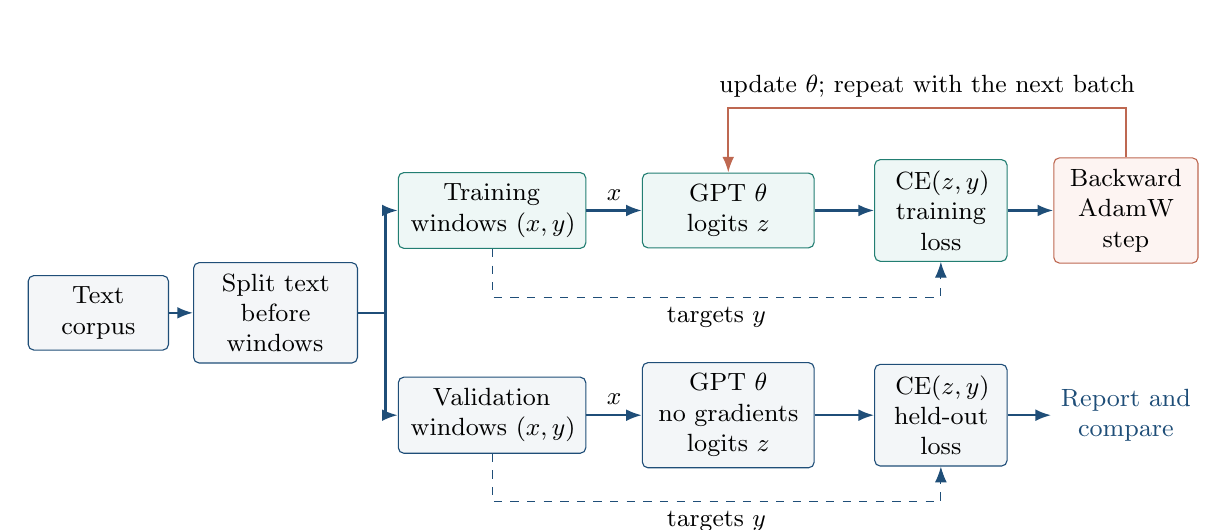
\begin{tikzpicture}[
  font=\small,
  flow/.style={-{Latex[length=2mm]},thick,draw=navy},
  target/.style={-{Latex[length=2mm]},draw=navy,dashed},
  update/.style={-{Latex[length=2mm]},thick,draw=coral!85!black},
  box/.style={draw=navy,fill=navy!5,rounded corners=2pt,
    align=center,minimum height=0.88cm,inner sep=4pt},
  train/.style={box,draw=teal!80!black,fill=teal!8},
  check/.style={box,draw=navy,fill=codebg}
]
\node[box,text width=1.5cm] (corpus) at (1,0) {Text\\corpus};
\node[box,text width=1.8cm] (split) at (3.25,0) {Split text\\before windows};
\node[train,text width=2.1cm] (trainwin) at (6,1.3)
  {Training\\windows $(x,y)$};
\node[check,text width=2.1cm] (valwin) at (6,-1.3)
  {Validation\\windows $(x,y)$};
\node[train,text width=1.9cm] (trainmodel) at (9,1.3)
  {GPT $\theta$\\logits $z$};
\node[check,text width=1.9cm,minimum height=1.08cm] (valmodel) at (9,-1.3)
  {GPT $\theta$\\no gradients\\logits $z$};
\node[train,text width=1.4cm] (trainloss) at (11.7,1.3)
  {$\mathrm{CE}(z,y)$\\training loss};
\node[check,text width=1.4cm] (valloss) at (11.7,-1.3)
  {$\mathrm{CE}(z,y)$\\held-out loss};
\node[train,text width=1.55cm,draw=coral!85!black,fill=coral!8]
  (optim) at (14.05,1.3) {Backward\\AdamW step};
\node[align=center,text width=1.65cm,text=navy] (report) at (14.05,-1.3)
  {Report and\\compare};

\draw[flow] (corpus) -- (split);
\draw[flow] (split.east) -- ++(0.35,0) |- (trainwin.west);
\draw[flow] (split.east) -- ++(0.35,0) |- (valwin.west);
\draw[flow] (trainwin) -- node[above] {$x$} (trainmodel);
\draw[flow] (valwin) -- node[above] {$x$} (valmodel);
\draw[flow] (trainmodel) -- (trainloss);
\draw[flow] (valmodel) -- (valloss);
\draw[flow] (trainloss) -- (optim);
\draw[flow] (valloss) -- (report);

% Shifted target IDs go directly to the loss, not into the decoder input.
\draw[target] (trainwin.south) -- (6,0.2)
  -- node[below] {targets $y$} (11.7,0.2) -- (trainloss.south);
\draw[target] (valwin.south) -- (6,-2.4)
  -- node[below] {targets $y$} (11.7,-2.4) -- (valloss.south);
\draw[update] (optim.north) -- (14.05,2.6)
  -- node[above] {update $\theta$; repeat with the next batch} (9,2.6)
  -- (trainmodel.north);
\end{tikzpicture}
\caption{The pretraining data and optimization paths. Split the corpus before
forming overlapping windows, tokenize each split with the same fixed tokenizer,
and shift each window by one position to obtain input IDs $x$ and target IDs $y$.
Cross-entropy (CE) compares the logits with the targets. Only the training branch
computes gradients and updates parameters. Validation uses the same current
parameters in evaluation mode, with dropout disabled and no gradient recording.
If the tokenizer is learned from the course corpus, fit it only on the training
split.}
\label{fig:pretraining-flow}
\end{figure}


\subsection{From a sequence probability to a trainable loss}
The probability chain rule is exact:
\[
p(x_1,\ldots,x_T)=\prod_{t=1}^{T}p(x_t\mid x_{<t}).
\]
The model approximates these conditional distributions using a finite context
and shared parameters $\theta$. A training input window $(x_1,\ldots,x_T)$ has
labels $(x_2,\ldots,x_{T+1})$. For its observed next tokens, maximizing the
product of conditional probabilities is equivalent to maximizing their summed
logarithms, hence to minimizing negative log-likelihood:
\begin{align*}
\arg\max_\theta\prod_{b,t}p_\theta(y_{bt}\mid x_{b,\le t})
&=\arg\max_\theta\sum_{b,t}\log p_\theta(y_{bt}\mid x_{b,\le t}),\\
\mathcal L_{\rm LM}(\theta)
&=-\frac{1}{BT}\sum_{b=1}^{B}\sum_{t=1}^{T}
\log p_\theta(y_{bt}\mid x_{b,\le t}).
\end{align*}
In these full-length pretraining windows every target contributes. Later, padding
or assistant-only training replaces $BT$ by the number of included targets and
omits masked terms. Such loss masks are different from the attention mask.

Training uses \emph{teacher forcing}: each position sees the observed earlier
tokens even if the model would have generated something else. All positions
can be evaluated in parallel because causal attention blocks future inputs.
Generation instead appends the model's own selected tokens. Errors may then
change the prefixes encountered later in the rollout.

\subsection{Logits, target probability, and cross-entropy}
Let $z_{btj}$ be the raw logit for vocabulary item $j$. For one target ID $y$,
\[
p_j=\frac{e^{z_j}}{\sum_{k=0}^{V-1}e^{z_k}},\qquad
\ell(z,y)=-\log p_y
=\log\left(\sum_{k=0}^{V-1}e^{z_k}\right)-z_y.
\]
The last expression connects the next-token objective to cross-entropy against
the one-hot target distribution. Implement the combined operation with
\texttt{cross\_entropy}; do not explicitly exponentiate large logits, take a
logarithm of a rounded probability, or pass softmax probabilities to that API.

For example, if the model assigns its three correct next tokens probabilities
$1/2$, $1/4$, and $1/8$, their mean loss is
\[
-\tfrac13\left(\log\tfrac12+\log\tfrac14+\log\tfrac18\right)
=\log4\approx1.3863.
\]
This is a constructed numerical example, not a measured training result.
For a single logit vector the derivative is
\[
\frac{\partial\ell}{\partial z_j}=p_j-\mathbf1\{j=y\}.
\]
Thus gradient descent increases the correct token's score relative to the
others, while backpropagation adjusts every upstream component that contributed
to these logits. Autograd performs this chain rule; it does not choose targets,
the loss, or the optimizer for us.

\begin{lstlisting}[language=Python]
import torch
from torch.nn import functional as F

def loss_batch(model, x, y):
    logits = model(x).logits  # book: logits = model(x)
    # logits: (B, T, V), y: (B, T), integer next-token IDs
    return F.cross_entropy(logits.flatten(0, 1), y.flatten())
\end{lstlisting}
The flattening creates $BT$ classification events over $V$ classes. It does
not mix time steps within a target and does not shift labels. A second shift
here would train the wrong prediction task.

\subsection{What perplexity measures}
For natural-log loss, $\operatorname{PPL}=\exp(\mathcal L)$. The example above
has perplexity $4$, the inverse geometric mean of the three correct-token
probabilities. A uniform predictor has loss $\log V$ and perplexity $V$.
A randomly initialized network need not be exactly uniform.

Perplexity is not accuracy and does not count the literal number of plausible
words. It depends on token boundaries, the held-out text, the context policy,
and which targets are scored. Compare it only under the same evaluation
protocol. Mean token loss should be exponentiated once; averaging per-batch
perplexities is a different quantity.

\subsection{The book's small corpus and split}
Raschka's chapter-5 example uses Edith Wharton's short story \emph{The Verdict}.
The exact course-reading download source is the pinned
\booklink{ch02/01_main-chapter-code/the-verdict.txt}{repository text file};
the raw endpoint is linked in the source records at the end of these notes.
The demonstration divides the raw text at 90\% of its character length,
tokenizes the two pieces separately with the fixed GPT-2 tokenizer, and then
constructs windows. This prevents overlapping windows from crossing the split,
but the two sets still come from the same story. It is not a held-out-author
or held-out-book generalization experiment.

The chapter-5 notebook uses context length and stride $256$, batch size $2$,
training shuffle enabled, and incomplete training batches dropped. Validation
does not shuffle and does not drop the last batch. An epoch is one pass through
the resulting training loader, not one pass through every possible overlapping
window or every possible prefix length.

\subsection{Evaluation must change both mode and gradient tracking}
\texttt{model.eval()} disables dropout; it does not disable autograd.
\texttt{torch.no\_grad()} disables graph recording; it does not disable dropout.
Use both to measure loss with fixed model parameters and deterministic network
layers. Restore the previous mode afterward.

The book's \texttt{calc\_loss\_loader} averages batch means over at most
\texttt{eval\_iter} batches. That is an exact token mean when batches contain
the same number of scored targets. The following original course adaptation
weights by token count so an incomplete final batch is handled correctly.
It assumes dense pretraining labels, with no padding or ignored targets.

\begin{lstlisting}[language=Python]
@torch.no_grad()
def evaluate(model, loader, device, max_batches=None):
    was_training = model.training
    model.eval()
    total_nll, total_tokens = 0.0, 0
    try:
        for i, (x, y) in enumerate(loader):
            if max_batches is not None and i >= max_batches:
                break
            x, y = x.to(device), y.to(device)
            logits = model(x).logits  # book: model(x)
            total_nll += F.cross_entropy(
                logits.flatten(0, 1), y.flatten(),
                reduction="sum").item()
            total_tokens += y.numel()
    finally:
        model.train(was_training)
    if total_tokens == 0:
        raise ValueError("No validation targets were scored")
    return total_nll / total_tokens
\end{lstlisting}

When \texttt{max\_batches=5}, five is a maximum, not a guarantee. In the book's
short-story example the validation loader is smaller than that. Partial-loader
or sampled-window evaluation is a useful progress estimate, but must not be
reported as an exhaustive corpus evaluation. Reusing validation to choose
hyperparameters makes it a model-selection set; reserve a separate test set for
a final claim.

\section{Pretraining: the first training loop, chapter 5.2}
\label{sec:basic-loop}

\subsection{Start with one device and one optimizer step per batch}
The first loop should expose the essential computation before adding a schedule,
mixed precision, gradient accumulation, or multiple GPUs:
\begin{enumerate}
\item Obtain integer inputs $X$ and already-shifted targets $Y$.
\item Compute raw logits and the mean cross-entropy.
\item Clear old gradients, backpropagate this batch's loss, and update parameters.
\item Periodically evaluate and record the number of processed token positions.
\item Inspect continuations from a fixed prompt after each epoch.
\end{enumerate}
Clearing gradients is necessary because PyTorch accumulates them by default.
\texttt{backward()} computes gradients but does not change parameter values;
\texttt{optimizer.step()} makes the update. For plain gradient descent this is
$\theta\leftarrow\theta-\eta\nabla\mathcal L$. AdamW additionally tracks first
and second gradient moments and applies decoupled weight decay.

The \emph{chapter notebook} uses AdamW with learning rate $4\times10^{-4}$,
weight decay $0.1$, ten epochs, and evaluation every five updates using at most
five batches per loader. It seeds PyTorch before constructing the model.
The compact \texttt{gpt\_train.py} summary uses different defaults
($5\times10^{-4}$ and one evaluation batch); do not mix those settings and call
the result the notebook experiment. The original short-story setup has a large
model relative to its data and intentionally exposes overfitting.

\begin{lstlisting}[language=Python]
def train_basic(model, train_loader, val_loader, device,
                epochs=10, eval_every=5):
    model.to(device)
    optimizer = torch.optim.AdamW(
        model.parameters(), lr=4e-4, weight_decay=0.1)
    history, tokens_seen, updates = [], 0, 0
    for epoch in range(epochs):
        model.train()
        for x, y in train_loader:
            x, y = x.to(device), y.to(device)
            optimizer.zero_grad(set_to_none=True)
            loss = loss_batch(model, x, y)
            if not torch.isfinite(loss):
                raise RuntimeError("Non-finite training loss")
            loss.backward()
            optimizer.step()
            tokens_seen += y.numel()
            updates += 1
            if updates == 1 or updates % eval_every == 0:
                train_nll = evaluate(model, train_loader,
                                     device, max_batches=5)
                val_nll = evaluate(model, val_loader,
                                   device, max_batches=5)
                history.append((updates, tokens_seen,
                                train_nll, val_nll))
        # Inspect a fixed-prompt continuation here; see below.
    return history, optimizer
\end{lstlisting}
This is an original condensed loop with the course \texttt{GPTOutput} interface,
not a verbatim copy of the book. It uses one-based update numbers; the book's
zero-based \texttt{global\_step=0} already follows its first optimizer update.
For a fresh run, set the seed \emph{before} creating the model, loaders, and
optimizer. An evaluation before the loop is useful as a genuine untrained
baseline. Calling the first post-update measurement ``initial loss'' would
confuse these two points in time.

\subsection{Reading training curves without overclaiming}
Compare train and validation loss with dropout disabled and the same scoring
convention. Falling train loss with rising held-out loss is evidence of
overfitting under that protocol. Similar losses can be entirely healthy; they
do not alone prove leakage. A nearly constant loss may reflect an incorrect
target shift, missing updates, unsuitable learning rate, or too little training.
Inspect these mechanisms before scaling the model.

The course's \emph{production-style driver} logs the just-used training batches
with dropout before an update, and evaluates sampled validation batches without
dropout after it. Those two logged values are not a clean matched estimate of
the generalization gap. Its validation batches also change over time. Use a
fixed held-out scoring protocol for comparisons that need finer precision.

\begin{studybox}{A useful small experiment}
Overfit one small batch to test whether the network and optimizer can reduce
its loss. Then evaluate on text never used for updates. Success on the repeated
batch is a correctness diagnostic, not generalization evidence. Compare several
fixed-prompt continuations, not only the most fluent one. Keep the tokenizer,
prompt, context length, and decoding settings fixed across checkpoints.
\end{studybox}

\section{From a checkpoint to text: chapters 5.3--5.4}
\label{sec:book-generation}

\subsection{Greedy decoding, temperature, and top-k}
For a prompt of length $t$, run the last $\min(t,C)$ IDs through the decoder.
The vector \texttt{logits[:, -1, :]} predicts the next ID. Select that ID, append
it, and repeat. Earlier output positions are useful for parallel training but
do not predict the next token after the entire current prompt.

Greedy decoding chooses $\arg\max_j z_j$. For $\tau>0$, temperature sampling uses
\[
p_j=[\softmax(z/\tau)]_j,\qquad
x_{t+1}\sim\operatorname{Categorical}(p).
\]
Lower temperature concentrates probability and higher temperature flattens it.
Changing a positive temperature cannot change the greedy argmax ordering.
It can change a sampled sequence, but does not guarantee a different realized
draw. Top-$k$ keeps the largest $k$ scores and masks the rest before normalizing.
At $k=1$ this is effectively greedy when the maximum is unique.

\begin{lstlisting}[language=Python]
@torch.no_grad()
def sample_next(model, ids, context_size, vocab_size,
                temperature=1.0, top_k=40):
    if temperature <= 0:
        raise ValueError("Use argmax for greedy decoding")
    if not 1 <= top_k <= vocab_size:
        raise ValueError("top_k must be within the vocabulary")
    if vocab_size > model.config.vocab_size:
        raise ValueError("Tokenizer is larger than the model")
    was_training = model.training
    model.eval()
    try:
        z = model(ids[:, -context_size:]).logits[:, -1, :]
        z = z[:, :vocab_size] / temperature
        values, indices = torch.topk(z, top_k, dim=-1)
        filtered = torch.full_like(z, -torch.inf)
        filtered.scatter_(1, indices, values)
        return torch.multinomial(filtered.softmax(-1), 1)
    finally:
        model.train(was_training)
\end{lstlisting}
This course-interface snippet selects one token; call it repeatedly and
concatenate its return value along dimension 1. It intentionally recomputes the
cropped context and has no key/value cache. It assumes a nonempty prompt,
$1\le\texttt{context\_size}\le C$, valid input IDs, and finite logits. The
full CLI additionally handles checkpoint/tokenizer validation and stopping.
Released GPT-2 token IDs cannot be substituted for the course tokenizer's IDs.

\subsection{Saving weights versus resuming training}
Chapter 5.4 first saves and reloads \texttt{model.state\_dict()}, then includes
optimizer state for continued training. Reconstruct the same model configuration
before loading its weights. For inference, select evaluation mode and pair it
with the exact tokenizer. Loading only weights and creating a new optimizer is
a fresh optimizer trajectory, even if the parameter values are unchanged.

A course checkpoint records configuration, model state, optimizer state, update
number, and metadata including the tokenizer identity. It does \emph{not} yet
provide exact restart: the current pretraining CLI has no resume option and its
payload omits RNG, batch-generator, and GradScaler states. An exact-resume
implementation would also restore the schedule position and data-order state.
Only load checkpoint files from a trusted source because general serialized
PyTorch payloads can execute code when deserialized.

\subsection{The boundary of ``from scratch''}
Chapter 5.5 separately demonstrates loading released OpenAI GPT-2 weights.
That is a useful architecture-compatibility exercise, not a result obtained by
training on \emph{The Verdict}. The course's pretraining exercise starts from
random weights and does not require that step. Similarly, useful instruction
following is a later objective rather than an automatic consequence of a
working next-token training loop.

\begin{studybox}{Pretraining checkpoint questions}
Can you explain every dimension from input IDs to loss? Why must masking occur
before softmax? Why does \texttt{eval()} not replace \texttt{no\_grad()}?
What is counted by ``tokens seen''? What would make two perplexities comparable?
Which states would you restore to resume training exactly? Answer these before
adding the larger-corpus and hardware extensions in the next sections.
\end{studybox}


\section{Course extension: data, leakage, and the public-book experiment}
\label{sec:corpus}

The downloader obtains English text records from Project Gutenberg's official
weekly compressed CSV catalog rather than a fixed title list. It removes the
separate homework title and normalized-title duplicates, randomly samples the
requested N works, and assigns about 10\% to validation as whole books. Thus an
evaluation window cannot be the next paragraph after a training window from the
same file.

Selection is also cache-aware. Nonempty files already named
\texttt{raw/books/pg<ID>.txt} are shuffled ahead of missing candidates. Raising
\texttt{--book-limit} from $N$ to $M$ needs $M-N$ new successful downloads when
there are exactly $N$ usable, eligible cached books. Larger caches or changes in
catalog eligibility can change that number. Selected nonempty cached files are
not downloaded again. This cache-first policy is randomized, but is not uniform
sampling from the entire eligible catalog on every invocation.
There is no hard-coded upper cap: the limit must be at least two and no larger
than the eligible population in the current catalog.

The manifest records the generated or user-supplied random seed, cached catalog
SHA-256, exact active selection and whole-book split, reuse/download counts,
resolved archive URLs, and hashes. Preparation reads that manifest and writes
token arrays one book at a time. New payloads use a registered high-speed
mirror's text files or archives with a two-second delay; bulk automation must not
target the human-facing site. A private or authorized mirror URL template can be
supplied for very large collections.

Each downloader run assigns a new active selection and split. Preserve the
manifest and processed streams for the duration of an experiment rather than
rerunning selection midway through training. About 10\% of \emph{books} held
out does not imply 10\% of tokens: lengths vary substantially. The tokenizer is
fitted on a character-limited prefix of the training-book iterator in manifest
order. Downloading 10,000 books therefore does not automatically expose BPE
fitting to all of them. Choose and record the tokenizer character budget.

Preparation joins each split's books with end-of-text tokens. Random training
windows may cross a book boundary within one split, but never cross the separate
training and validation streams. The current binary format stores unsigned
16-bit IDs, so its vocabulary must fit that representation. Arbitrarily large
book counts do not imply arbitrarily large token IDs.

\begin{figure}[H]\centering
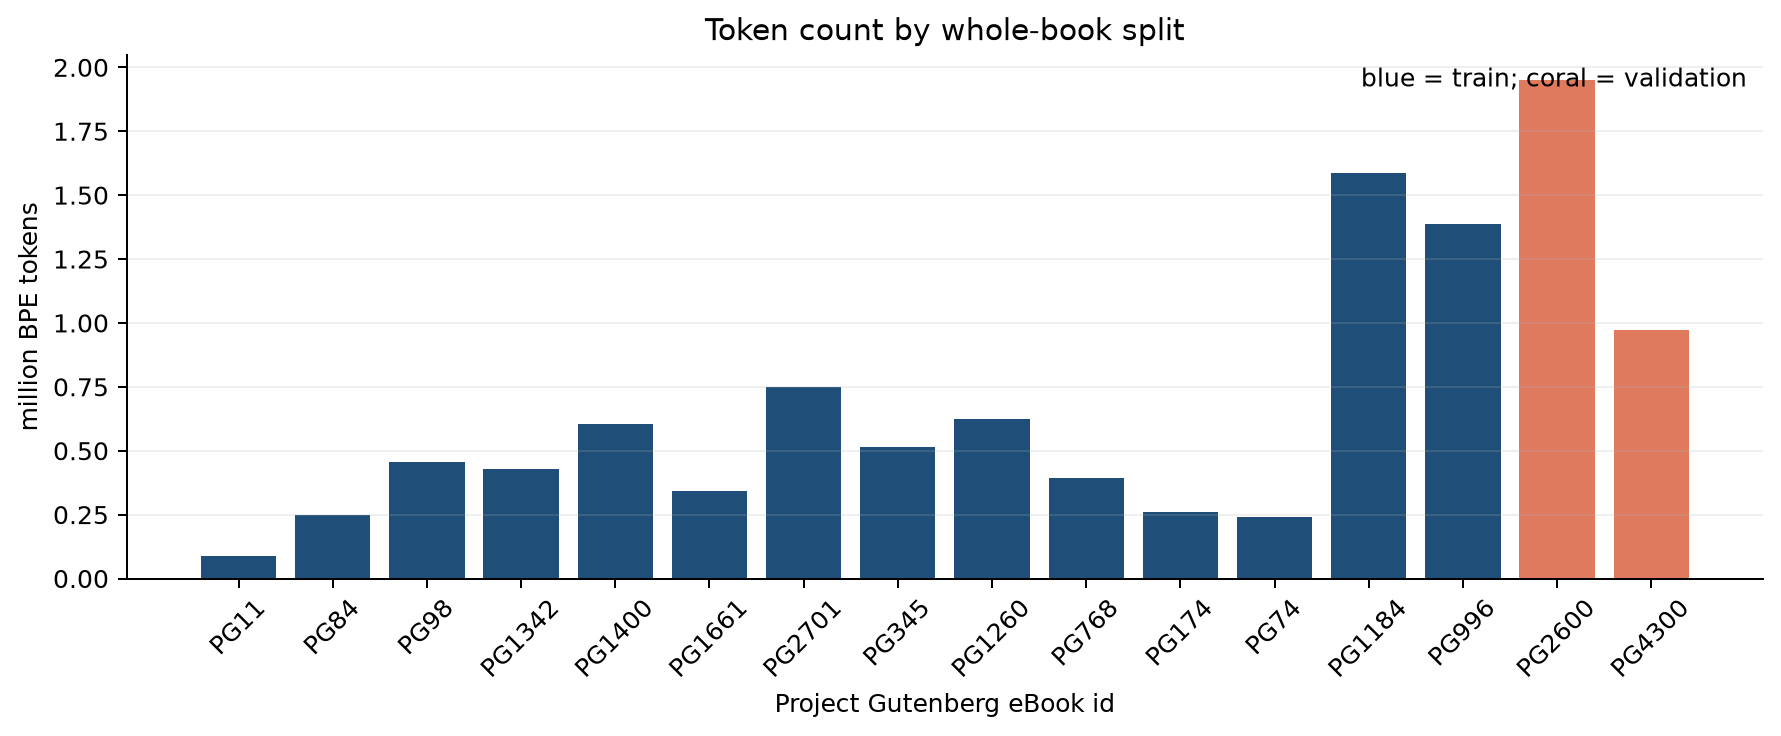
\includegraphics[width=0.96\linewidth]{corpus_tokens.png}
\caption{Earlier 16-book measurement; validation books were held out from tokenizer and model training.}
\end{figure}

The archived 16-book snapshot is English fiction with historical language and
outdated social assumptions. A new, much larger catalog selection need not have
the same genre composition, so inspect its manifest rather than inheriting that
description. Neither selection is automatically representative of contemporary
general-language use. The data route is
chosen for reproducibility, public accessibility, and scale appropriate for a
classroom accelerator -- not because it is an ethically or statistically ideal
foundation-model corpus.

\subsection{The bigram baseline and controlled comparisons}
The course baseline learns a logit row for each current token:
\[
p(x_{t+1}=j\mid x_t=i)=[\softmax(B_{i,:})]_j.
\]
It cannot use earlier context. Compare it with the decoder using the same
tokenizer, held-out documents, scoring rule, and declared training budget. If
the decoder does not improve held-out loss, investigate the implementation and
budget before attributing benefit to attention. This is a proposed comparison,
not a claimed result of the archived 30-update run.

\section{Course extension: optimization and hardware}
\label{sec:hardware}

The first chapter-5 loop needs none of the following additions. Raschka's
Appendix D introduces warmup, cosine decay, and gradient clipping after the
basic loop works. The course then adds accumulation, CUDA mixed precision,
checkpoint guards, and an optional distributed driver.

The course groups matrix parameters (weight decay) separately from bias and
normalization vectors (no decay). This is a parameter-group choice, not an
automatic behavior of AdamW. It uses moment coefficients $(0.9,0.95)$, whereas
the book's minimal constructor uses PyTorch's default $(0.9,0.999)$.
With zero-based optimizer update index $s$, total budget $S$, and warmup length
$s_w<S$, the implemented schedule is
\[
\eta_s=\begin{cases}
\eta_{\max}(s+1)/s_w,&0\le s<s_w,\\
\eta_{\min}+\tfrac12(\eta_{\max}-\eta_{\min})
\left[1+\cos\left(\pi\frac{s-s_w}{S-s_w}\right)\right],&s_w\le s<S.
\end{cases}
\]
When $s_w=0$, use only the cosine branch. The last executed index is $S-1$;
the minimum is the schedule's endpoint at $S$. Divide each microbatch mean loss
by accumulation count $A$ before backpropagation, then clip and update once
after $A$ equal-size microbatches. This gives the gradient of their average loss.
It is not generally bitwise identical to a larger physical batch with dropout.

The loop clips the total gradient norm, evaluates a fixed \emph{number} of fresh
random validation batches, saves best and periodic checkpoints, and raises on
nonfinite training or evaluation \emph{losses}. It does not explicitly reject
every nonfinite gradient before an update. The logged gradient norm is the norm
before clipping. \texttt{auto} selects CUDA, then
Apple MPS, then CPU. Explicit unavailable accelerators raise an error.
Only CUDA uses autocast in the current driver; FP16 gradient scaling is also
CUDA-only. Selecting a non-FP32 setting alone does not enable MPS mixed precision.

The default driver uses one device. The optional distributed driver is launched
by \texttt{torchrun}, which supplies a global rank, local rank, and world size.
Each process selects CUDA device \texttt{LOCAL\_RANK}, constructs one complete
model replica, and draws different token windows using a rank-offset seed. DDP
broadcasts the initial parameters and averages gradients across workers. During
gradient accumulation, \texttt{no\_sync()} defers communication until the final
microbatch. Validation losses are averaged with an all-reduce, while only rank
zero prints and writes checkpoints. Thus
\[
B_{\rm effective}=B_{\rm worker}\times A\times W,
\]
where $A$ is the accumulation count and $W$ the number of workers. DDP is data
parallelism, not model sharding: every GPU must fit the full parameters,
optimizer state, and its local activations. MPS remains single-device; the
multi-GPU classroom route uses CUDA with NCCL.

The token-position budget is $S\,B_{\rm worker}\,A\,W\,T$. These are prediction
events consumed by updates, including repeated sampled windows. They are not
unique tokens and do not certify a full corpus pass. The single-device driver
uses random starts with replacement rather than DataLoader epochs.

\begin{figure}[H]\centering
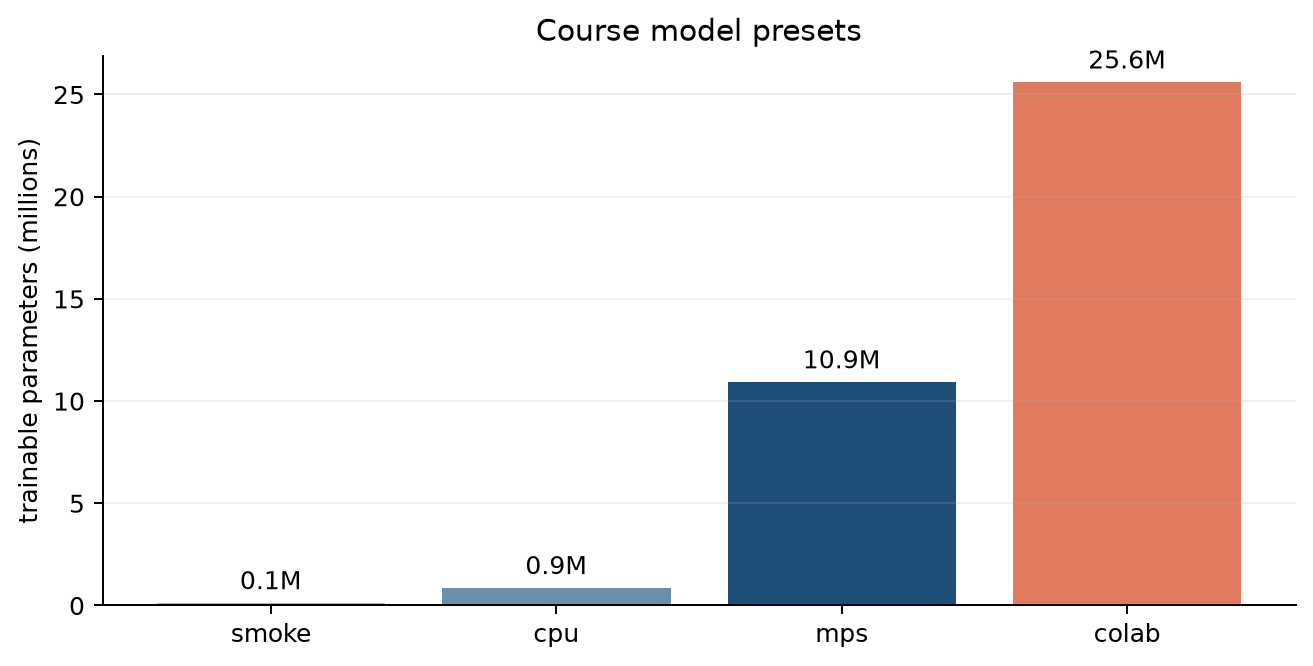
\includegraphics[width=0.75\linewidth]{preset_parameters.png}
\caption{Exact parameter counts at vocabulary size 512. Parameter count alone
does not predict training time; sequence length, batch, kernel support, and device matter.}
\end{figure}

The MPS preset is six layers, six heads, width 384, context 256, batch 16, and
6,000 updates: $24{,}576{,}000$ token positions at accumulation one. Vocabulary
size changes its parameter count; the figure's counts assume $V=512$.
Rather than promise a runtime, time 100 updates \emph{after} the 200-update
warmup on the actual machine and extrapolate, allowing for evaluation and saving.
The CLI's \texttt{--steps} changes only the total update budget: an MPS run with
\texttt{--steps 100} remains inside warmup.
Apple MPS performance varies by PyTorch/macOS version and memory pressure. Colab
GPU type is not fixed across sessions.

\begin{studybox}{Current reproducibility boundary}
Seed before model construction when designing a controlled experiment. The
current single-device pretraining driver constructs its GPT before the training
helper sets the global seed. Its preset seed therefore controls later training
randomness and batch generators, but does not guarantee identical initial
weights across fresh invocations. The minimal loop above should be called only
after deliberate initialization seeding. The CLI also has no exact-resume path;
use a fresh checkpoint root for each run and record its configuration.
\end{studybox}

\section{Course extension: decoding and tokenizer contracts}

At each step, crop to the last $T_{\max}$ tokens, compute the final-position
logits $z$, divide by temperature $\tau$, optionally keep only the top $k$, and
sample:
\[
p_i=[\softmax(z/\tau)]_i,\qquad x_{t+1}\sim\operatorname{Categorical}(p).
\]
Low temperature concentrates mass; high temperature flattens the distribution
before truncation. Whether a change improves text quality is empirical.
Top-$k$ truncation removes the long tail but can also suppress rare valid
tokens. Report the prompt, seed, temperature, truncation rule, and checkpoint.
Never present one appealing sample as a distributional evaluation.

The generation CLI now draws a fresh 32-bit seed for each unseeded invocation
and prints it to standard error. Repeated commands therefore use fresh random
streams by default, though they may still generate identical text. Pass
\texttt{--seed 2026} for controlled repeats in the same environment; bitwise
identity across devices and software versions is not guaranteed.
Temperature changes the probabilities but does not mathematically
guarantee that one finite draw differs from another; seed controls the random
draw, while temperature controls its distribution.

Generation must also respect the tokenizer boundary. Let $V_{\rm tok}$ be the
actual tokenizer size and $V_{\rm model}$ the number of model output rows. The
valid next-token distribution is
\[
p_i=\softmax\!\left(z_{0:V_{\rm tok}}/\tau\right)_i,
\qquad 0\le i<V_{\rm tok}\le V_{\rm model}.
\]
The implementation slices logits before top-$k$ and sampling, so intentionally
padded rows cannot be drawn. New checkpoints also record the tokenizer size and
SHA-256. A conflicting tokenizer file raises an early error; use
\texttt{--tokenizer data/llm/processed/tokenizer.json} to select the exact file
used for training rather than hiding a stale sidecar as padding.
The training drivers stage this tokenizer beside the checkpoints before the
first update and refuse to mix existing checkpoints with a different tokenizer.
When changing BPE settings, select a fresh checkpoint root or output directory.

Legacy checkpoints without a stored tokenizer hash cannot automatically detect
every wrong same-size mapping. A matching vocabulary size alone is insufficient.
Never repair a mapping mismatch by silently dropping or replacing generated IDs.

The archived 30-update public-book smoke checkpoint produced mostly
character-like noise even though held-out loss fell from 6.207 after update 1
to 5.126 after update 30. These are not measurements of the user's later
10,000-book run. This is expected and useful:
optimization correctness is a necessary condition for language learning, not a
sufficient condition.

\clearpage
\part{Post-training extensions}
\section{Supervised instruction fine-tuning}

The remaining lessons keep the original course's SFT, reward-model, and PPO
material. They are not prerequisites of chapters 2--5. Raschka's chapter 7
provides a next reading on instruction fine-tuning; the Dolly data, assistant-only
loss choice, HH-RLHF preferences, and PPO implementation below are course
extensions rather than a description of the book's pretraining experiment.

A base model learns continuation, not the social convention ``answer the user.''
SFT formats each Dolly record as system text, user instruction and optional
context, then assistant response. Labels are shifted by one token, but prompt and
padding positions are set to $-100$, PyTorch's ignored target:
\[
\mathcal L_{\mathrm{SFT}}
=-\frac{1}{\sum_t m_t}\sum_t m_t
\log p_\theta(y_t\mid x,y_{<t}),
\quad m_t=\mathbf{1}\{t\text{ is assistant response}\}.
\]
Assistant-only masking concentrates this objective on response tokens.
Training on prompt tokens is another possible objective, not automatically a
bug, but long prompts then receive substantial weight. State the choice and
inspect the labels rather than interpreting every decrease as better answering.

Dolly 15k is human-authored and licensed CC BY-SA 3.0, but it is neither a truth
oracle nor a safety benchmark. Some answers are incomplete or wrong, contexts
can come from Wikipedia, and annotator demographics shape the distribution.
Evaluation should include a held-out split by record, task-category summaries,
response length, exact formatting checks, and human review.

\section{Pairwise reward modeling}

HH-RLHF provides conversations with a chosen and rejected answer. A reward model
uses the SFT GPT backbone and maps the final non-padding hidden state to a scalar
$r_\phi(x,y)$. Under the Bradley--Terry model,
\[
P(y^+\succ y^-\mid x)=\sigma(r_\phi(x,y^+)-r_\phi(x,y^-)),
\]
so the pair loss is $-\log\sigma(r^+-r^-)$. Pair accuracy is intuitive but can
hide calibration and distribution shift. Rewards are identifiable only up to an
additive constant; only differences matter for the likelihood.

HH-RLHF's harmless subset intentionally includes harmful prompts, slurs, unsafe
instructions, and rejected harmful answers. It is suitable for a controlled
safety lesson, not unfiltered projection or casual browsing. Dataset preferences
also reflect a particular policy and period; they do not define universal human
values.

\section{PPO-style RLHF}

The RL loop treats the prompt as initial state, generated tokens as actions, and
the reward-model score as a terminal reward. A frozen reference policy penalizes
drift. For sampled action $a_t$,
\[
r_t^{\mathrm{KL}}=-\beta\left[
\log\pi_\theta(a_t\mid s_t)-\log\pi_{\mathrm{ref}}(a_t\mid s_t)\right].
\]
Add the scalar reward-model score to the final generated action. This sampled log
ratio is a Monte Carlo contribution to forward KL; it is not the exact full-
vocabulary KL at every state.

Given values $V_t$, temporal-difference residuals and GAE are
\begin{align*}
\delta_t &= r_t+\gamma V_{t+1}-V_t,\\
\hat A_t &= \delta_t+\gamma\lambda\hat A_{t+1},\\
\hat R_t &= \hat A_t+V_t.
\end{align*}
With ratio $\rho_t=\exp(\log\pi_\theta-\log\pi_{\mathrm{old}})$, PPO minimizes the
negative clipped surrogate plus clipped value error and an entropy bonus:
\[
\mathcal L_{\mathrm{policy}}=-\E_t\min\left(
\rho_t\hat A_t,
\operatorname{clip}(\rho_t,1-\epsilon,1+\epsilon)\hat A_t
\right).
\]

The code masks prompt and padding positions in every RL term. It logs mean reward,
approximate KL, policy loss, value loss, and clip fraction. A rising learned
reward with worsening human judgment is reward hacking, not success. Stop or
retune when KL spikes, response length collapses, phrases repeat, or held-out
human preference declines.

\section{Measured evidence and interpretation}
\begin{figure}[H]\centering
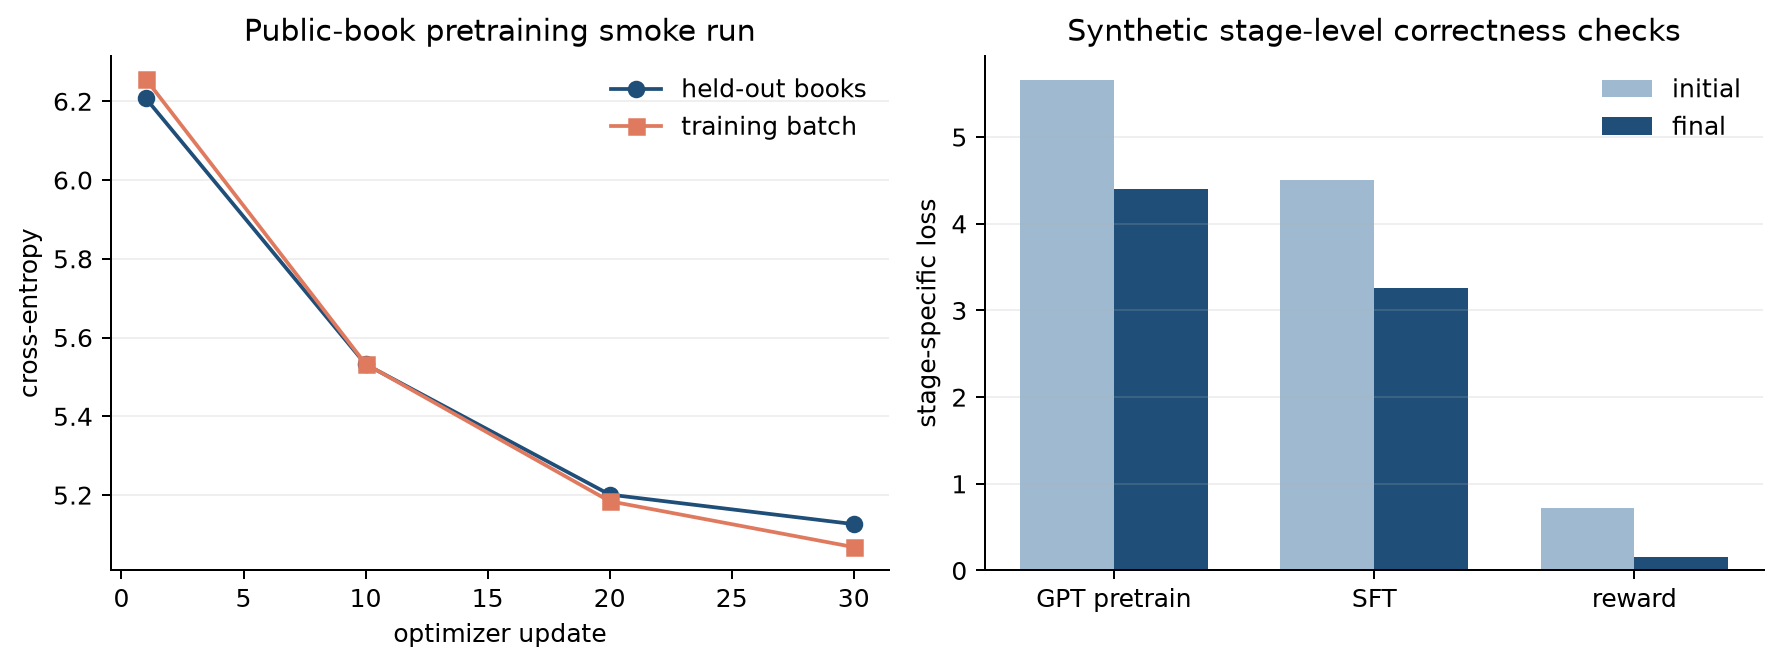
\includegraphics[width=0.98\linewidth]{training_evidence.png}
\caption{Left: genuine held-out-book pretraining. Right: synthetic correctness
checks whose losses have different semantics and must not be compared across stages.}
\end{figure}

The integrated CPU smoke run verifies all stages. The tiny GPT held-out loss falls
from 5.655 to 4.404; assistant-only SFT loss falls from 4.503 to 3.258; pairwise
reward loss falls from 0.717 to 0.159 on four pairs; PPO policy and value gradients
are finite. The reward model obtains 100\% accuracy on those same four pairs,
which demonstrates deliberate overfitting in a unit-sized test, not generalization.

\clearpage
\section{Failure modes and audit checklist}
\begin{longtable}{@{}P{0.24\linewidth}P{0.34\linewidth}P{0.34\linewidth}@{}}
\toprule
Symptom & Likely cause & Check or response \\
\midrule
\endhead
Unexpectedly strong validation on near-duplicates & possible document or tokenizer leakage & audit duplicates and split before windows; similar losses alone are not proof \\
Past logits change when future tokens change & missing/misaligned causal mask & behavioral causality unit test \\
SFT loss falls but answers do not improve & prompt tokens dominate & inspect $-100$ labels and token counts \\
Reward accuracy is high only on train & memorization or template cue & held-out prompts and source split \\
Reward rises, language degrades & reward hacking & human audit, KL limit, stop run \\
PPO KL explodes & learning rate or reward scale too large & lower rate/reward, raise KL penalty \\
MPS out of memory & context/batch too large & lower batch; accumulate gradients \\
One sample looks excellent & selection bias & fixed prompt suite and distributional metrics \\
Every command emits the same sample & fixed seed, greedy decoding, or concentrated probabilities & inspect seed, temperature, top-$k$, and logits \\
Decoder reports an out-of-vocabulary ID & padded head or wrong tokenizer sidecar & mask to actual size; verify size/hash or pass \texttt{--tokenizer} \\
\bottomrule
\end{longtable}

Before making a claim, record data revision and license, tokenizer hash, model
configuration, seed, device, token budget, checkpoint, held-out protocol,
generation settings, failure examples, and the exact population to which the
claim is intended to generalize.

\section{Reproducible lab commands}
Use the existing prepared corpus if available. In particular, do not redownload
or retokenize a 10,000-book corpus merely to follow this lesson. Confirm that
\texttt{data/llm/processed/} contains \texttt{tokenizer.json},
\texttt{metadata.json}, \texttt{train.bin}, and \texttt{validation.bin}.
The metadata supplies the actual vocabulary size. These commands use a fresh
checkpoint root so the lecture exercise does not replace an earlier run.
\begin{lstlisting}[language=bash]
uv sync --locked --extra llm
make test-llm

# First verify the complete pipeline with a short run.
uv run --extra llm python -m experiments.llm.pretrain \
  --preset smoke --steps 30 --device auto \
  --checkpoint-root checkpoints/llm-lecture-revision

# Then choose a larger budget after measuring the actual hardware.
uv run --extra llm python -m experiments.llm.pretrain \
  --preset mps --device auto \
  --checkpoint-root checkpoints/llm-lecture-revision

# Omit --seed for a fresh reported seed; retain it for controlled repeats.
uv run --extra llm python -m experiments.llm.generate \
  checkpoints/llm-lecture-revision/pretrain-mps/best.pt \
  --prompt "Once upon a time" --temperature 0.8 --top-k 40 --seed 2026
\end{lstlisting}

Students without prepared data can use a separate small directory:
\begin{lstlisting}[language=bash]
uv run --extra llm python -m experiments.llm.download_data \
  --dataset books --data-root data/llm-lecture-revision \
  --book-limit 16 --selection-seed 2026

uv run --extra llm python -m experiments.llm.prepare_data \
  --data-root data/llm-lecture-revision --tokenizer bpe \
  --vocab-size 512 --tokenizer-characters 500000
\end{lstlisting}
For this directory, add \texttt{--data-root data/llm-lecture-revision} to the
pretraining command. A larger book limit and tokenizer budget are independent
choices. Use another checkpoint root when changing tokenizer settings.

The later stages use separate data preparation for Dolly and HH-RLHF. Consult
\texttt{docs/topics/llm.md} before the commands below. They are optional
post-training labs, not steps required for the chapter-5 exercise.
\begin{lstlisting}[language=bash]
# Optional CUDA data parallelism: one process per GPU.
uv run --extra llm torchrun --standalone --nproc_per_node=2 \
  -m experiments.llm.pretrain_distributed --preset colab --device cuda \
  --checkpoint-root checkpoints/llm-lecture-ddp

uv run --extra llm python -m experiments.llm.sft \
  checkpoints/llm-lecture-revision/pretrain-mps/best.pt --device auto \
  --output-dir checkpoints/llm-lecture-revision/sft

uv run --extra llm python -m experiments.llm.reward_modeling \
  checkpoints/llm-lecture-revision/sft/sft.pt --device auto \
  --output-dir checkpoints/llm-lecture-revision/reward

uv run --extra llm python -m experiments.llm.ppo \
  checkpoints/llm-lecture-revision/sft/sft.pt \
  checkpoints/llm-lecture-revision/reward/reward_model.pt --device auto \
  --output-dir checkpoints/llm-lecture-revision/ppo
\end{lstlisting}

\section{References and data records}
\subsection*{Primary reading and exact chapter code}
Sebastian Raschka, \emph{Build a Large Language Model (From Scratch)}, Manning,
2024, ISBN 9781633437166.
\href{https://www.manning.com/books/build-a-large-language-model-from-scratch}{Publisher page}.
The pretraining narrative follows the official chapter notebooks, with original
course explanations and condensed code examples. No book figures are reproduced.
\begin{itemize}
\item Chapter 2, especially sections 2.5--2.8:
\booklink{ch02/01_main-chapter-code/ch02.ipynb}{tokenization, shifted batches, embeddings}.
\item Chapter 3, sections 3.3--3.6:
\booklink{ch03/01_main-chapter-code/ch03.ipynb}{attention, masking, multiple heads}.
\item Chapter 4, sections 4.2--4.7:
\booklink{ch04/01_main-chapter-code/ch04.ipynb}{decoder components and generation};
\booklink{ch04/01_main-chapter-code/gpt.py}{compact GPT source}.
\item Chapter 5, sections 5.1--5.4:
\booklink{ch05/01_main-chapter-code/ch05.ipynb}{loss, training, sampling, saving};
\booklink{ch05/01_main-chapter-code/gpt_train.py}{training-script companion}.
Section 5.5's external weight-loading exercise is separate from random-initialized pretraining.
\item Appendix D:
\booklink{appendix-D/01_main-chapter-code/appendix-D.ipynb}{warmup, cosine decay, clipping}.
\item Chapter 7:
\booklink{ch07/01_main-chapter-code/ch07.ipynb}{optional instruction-tuning reading}.
\item Edith Wharton, \emph{The Verdict}:
\href{https://raw.githubusercontent.com/rasbt/LLMs-from-scratch/f49cad747931fe6af0a7d2802cd480d1c1a0ec8e/ch02/01_main-chapter-code/the-verdict.txt}{exact pinned raw-text download}.
\end{itemize}

\subsection*{Architecture, post-training, and data provenance}
\begin{itemize}
\item Sennrich, Haddow, and Birch (2016), BPE for subword units: \url{https://aclanthology.org/P16-1162/}.
\item Vaswani et al. (2017), Transformer attention: \url{https://arxiv.org/abs/1706.03762}.
\item Radford et al. (2019), GPT-2 report: \url{https://cdn.openai.com/better-language-models/language_models_are_unsupervised_multitask_learners.pdf}.
\item Ouyang et al. (2022), instruction following with human feedback: \url{https://arxiv.org/abs/2203.02155}.
\item Schulman et al. (2017), PPO: \url{https://arxiv.org/abs/1707.06347}.
\item Bai et al. (2022), helpful and harmless assistant: \url{https://arxiv.org/abs/2204.05862}.
\item Released GPT-2 architecture source:
\url{https://github.com/openai/gpt-2/blob/master/src/model.py}.
\item Karpathy, nanoGPT teaching and performance reference: \url{https://github.com/karpathy/nanoGPT}.
\item Project Gutenberg terms and permission: \url{https://www.gutenberg.org/policy/terms_of_use.html} and \url{https://www.gutenberg.org/policy/permission}.
\item Project Gutenberg official catalog and robot guidance: \url{https://www.gutenberg.org/ebooks/offline_catalogs.html} and \url{https://www.gutenberg.org/policy/robot_access.html}.
\item PyTorch documentation: \href{https://docs.pytorch.org/docs/stable/generated/torch.nn.parallel.DistributedDataParallel.html}{DistributedDataParallel} and \href{https://docs.pytorch.org/docs/stable/elastic/run.html}{\texttt{torchrun}}.
\item Exact item IDs, revisions, URLs, licenses, and checksums: \texttt{data/llm/sources.json} and the generated \texttt{data/llm/download\_manifest.json}.
\end{itemize}

\end{document}
